%%%%%%%%%%%%%%%%%%%%%%%%%%%%%%%%%%%%%%%%%
% The Legrand Orange Book
% LaTeX Template
% Version 3.1 (February 18, 2022)
%
% This template originates from:
% https://www.LaTeXTemplates.com
%
% Authors:
% Vel (vel@latextemplates.com)
% Mathias Legrand (legrand.mathias@gmail.com)
%
% License:
% CC BY-NC-SA 4.0 (https://creativecommons.org/licenses/by-nc-sa/4.0/)
%
% Compiling this template:
% This template uses biber for its bibliography and makeindex for its index.
% When you first open the template, compile it from the command line with the 
% commands below to make sure your LaTeX distribution is configured correctly:
%
% 1) pdflatex main
% 2) makeindex main.idx -s indexstyle.ist
% 3) biber main
% 4) pdflatex main x 2
%
% After this, when you wish to update the bibliography/index use the appropriate
% command above and make sure to compile with pdflatex several times 
% afterwards to propagate your changes to the document.
%
%%%%%%%%%%%%%%%%%%%%%%%%%%%%%%%%%%%%%%%%%

%----------------------------------------------------------------------------------------
%	PACKAGES AND OTHER DOCUMENT CONFIGURATIONS
%----------------------------------------------------------------------------------------

\documentclass[
	12pt, % Default font size, select one of 10pt, 11pt or 12pt
	fleqn, % Left align equations
	a4paper, % Paper size, use either 'a4paper' for A4 size or 'letterpaper' for US letter size
	%oneside, % Uncomment for oneside mode, this doesn't start new chapters and parts on odd pages (adding an empty page if required), this mode is more suitable if the book is to be read on a screen instead of printed
]{LegrandOrangeBook}

% Book information for PDF metadata, remove/comment this block if not required 
\hypersetup{
	pdftitle={A NEAT Inspired GEP Algorithm}, % Title field
	pdfauthor={Louis John Hassett, Duncan Anthony Coulter, Daniel Ogwok}, % Author field
	pdfsubject={Evolutionary Computing, Neural Networks}, % Subject field
	pdfkeywords={NEAT, GEP}, % Keywords
	pdfcreator={LaTeX}, % Content creator field
}

\addbibresource{main.bib} % Bibliography file

\definecolor{ocre}{RGB}{128, 0, 0} % Define the color used for highlighting throughout the book

\chapterimage{} % Chapter heading image
\chapterspaceabove{6.5cm} % Default whitespace from the top of the page to the chapter title on chapter pages
\chapterspacebelow{6.75cm} % Default amount of vertical whitespace from the top margin to the start of the text on chapter pages

%----------------------------------------------------------------------------------------
\usepackage{epigraph}
\usepackage[autostyle=true]{csquotes} % Required to generate language-dependent quotes in the bibliography
\usepackage{svg}
\usepackage{algorithm}
\usepackage{algpseudocode}
\usepackage{todonotes}


\linespread{1.5}
\begin{document}

%----------------------------------------------------------------------------------------
%	TITLE PAGE
%----------------------------------------------------------------------------------------

\titlepage % Output the title page
	{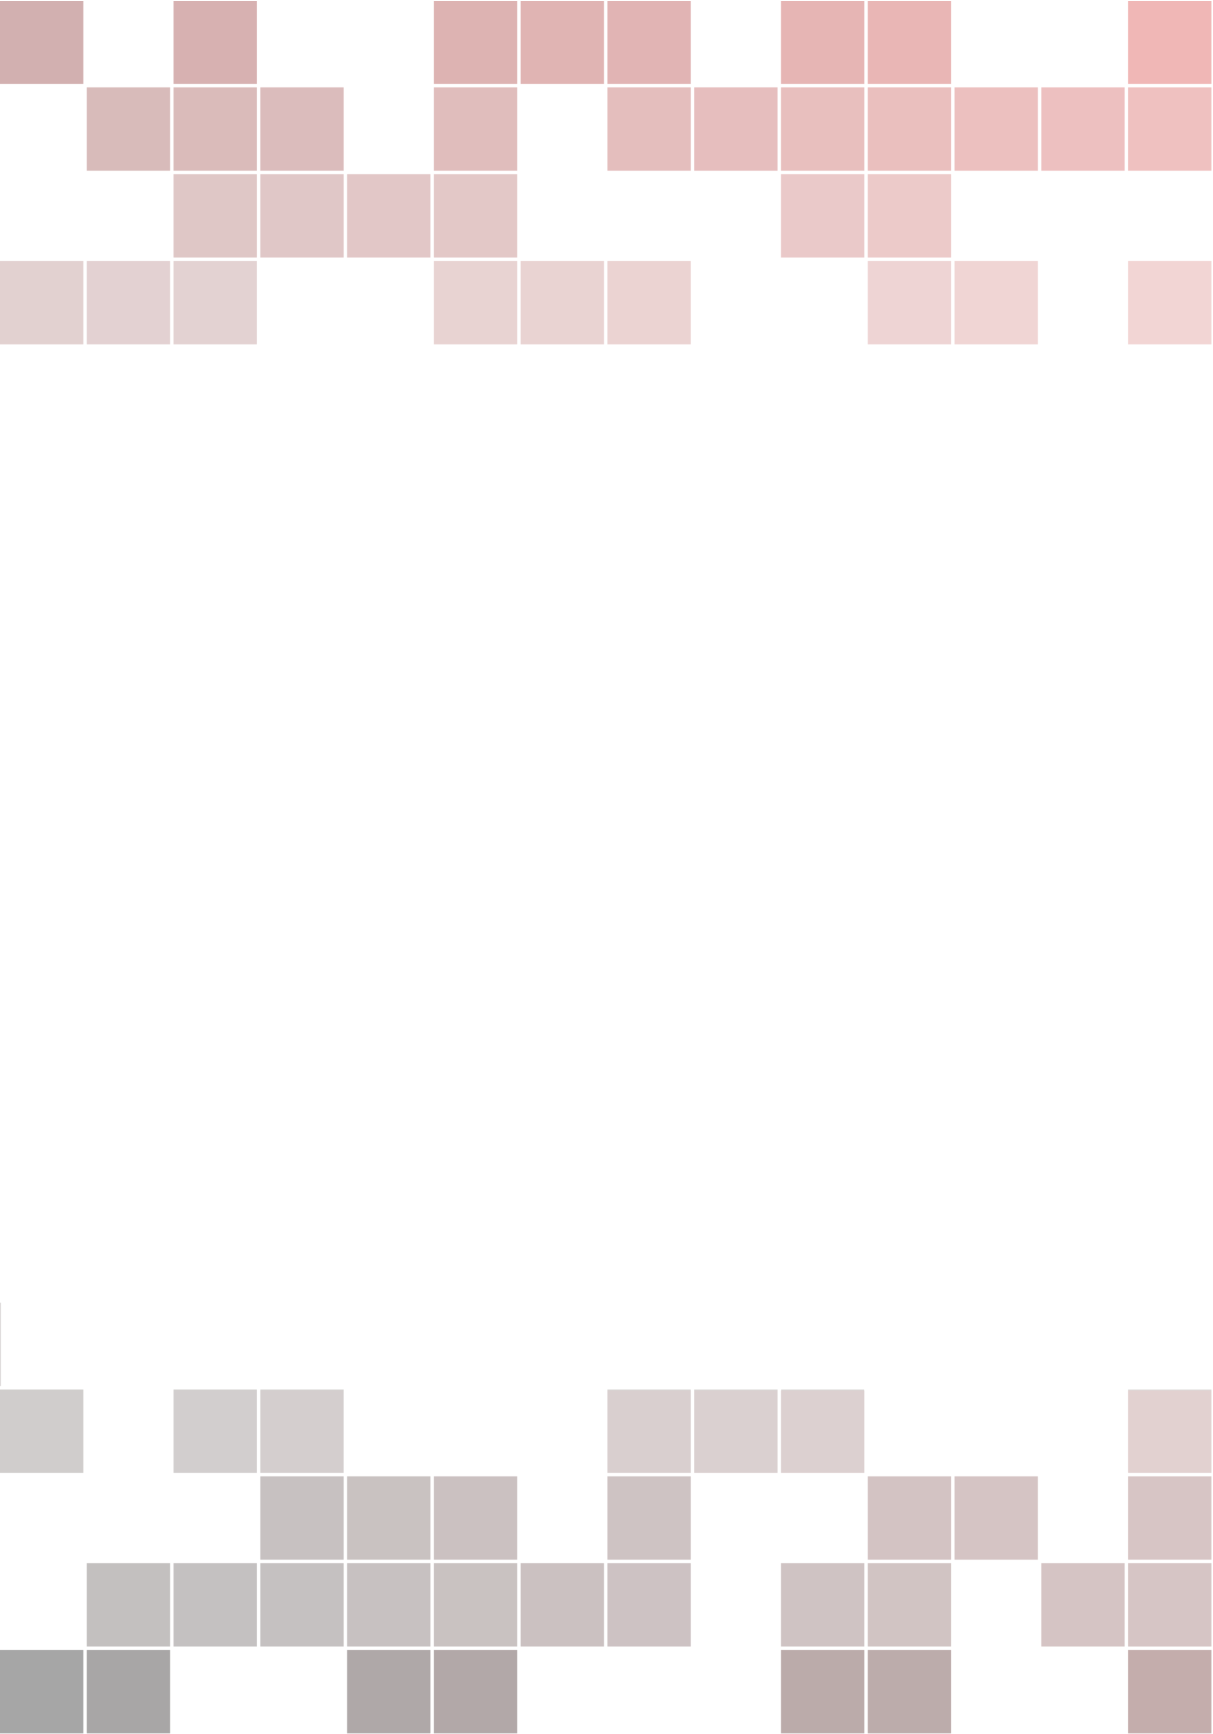
\includegraphics[width=\paperwidth]{background.pdf}} % Code to output the background image, which should be the same dimensions as the paper to fill the page entirely; leave empty for no background image
	{ % Title(s) and author(s)
		\centering\sffamily % Font styling
		{\LARGE \href{https://www.uj.ac.za/}{University of Johannesburg}\par} % Subtitle
		\vspace{16pt}
		{\large Masters Dissertation\par} % Subtitle
		\vspace{16pt} % Vertical whitespace
		{\Huge\bfseries A NEAT Inspired GEP Algorithm\par} % Book title
		\vspace{16pt} % Vertical whitespace
		% {\huge\bfseries Louis John Hassett\par} % Author name

		\begin{minipage}[t]{0.4\textwidth}
		\begin{flushleft} \large
		\emph{Author:}\\
		\href{http://www.johnsmith.com}{Louis John Hassett} % Author name - remove the \href bracket to remove the link
		\end{flushleft}
		\end{minipage}
		\begin{minipage}[t]{0.4\textwidth}
		\begin{flushright} \large
		\emph{Supervisor:} \\
		\href{http://www.jamessmith.com}{Prof. Duncan A. Coulter} \\ % Supervisor name - remove the \href bracket to remove the link  
		\emph{Co-supervisor:} \\
		\href{http://www.jamessmith.com}{Daniel Ogwok}
		\end{flushright}
		\end{minipage}\\[1cm]

		\large \textit{A dissertation submitted in fulfillment of the requirements\\ for the degree of Master in Computer Science}\\[0.3cm] % University requirement text
		\textit{in the}\\[0.4cm]
		\href{https://adam.uj.ac.za/academy/}{Faculty of Science\\Academy of Computer Science and Software Engineering}\\ % Research group name and department name
	}


%----------------------------------------------------------------------------------------
%	COPYRIGHT PAGE
%----------------------------------------------------------------------------------------

\thispagestyle{empty} % Suppress headers and footers on this page

\noindent\enquote{\itshape It is not the strongest of the species that survives, nor the most intelligent that survives. It is the one that is most adaptable to change. In the struggle for survival, the fittest win out at the expense of their rivals because they succeed in adapting themselves best to their environment.}\bigbreak

\hfill Charles Darwin


~\vfill % Push the text down to the bottom of the page

\noindent \textbf{Acknowledgements} \\
I would like to sincerely thank my supervisor, Prof Coulter, for his guidance and support throughout this research. His expertise and feedback were invaluable. 


%----------------------------------------------------------------------------------------
%	TABLE OF CONTENTS
%----------------------------------------------------------------------------------------

\pagestyle{empty} % Disable headers and footers for the following pages

\tableofcontents % Output the table of contents

\listoffigures % Output the list of figures, comment or remove this command if not required

\listoftables % Output the list of tables, comment or remove this command if not required

\pagestyle{fancy} % Enable default headers and footers again

\cleardoublepage % Start the following content on a new page

%----------------------------------------------------------------------------------------
%	PART
%----------------------------------------------------------------------------------------

\part{Part One}

%----------------------------------------------------------------------------------------
%	SECTIONING EXAMPLES CHAPTER
%----------------------------------------------------------------------------------------
\chapterimage{} % Chapter heading image
\chapterspaceabove{6.75cm} % Whitespace from the top of the page to the chapter title on chapter pages
\chapterspacebelow{7.25cm} % Amount of vertical whitespace from the top margin to the start of the text on chapter pages

%------------------------------------------------
\chapterimage{}
\chapterspaceabove{6.75cm} 
\chapterspacebelow{7.25cm}
\chapter{Introduction}\index{chapter:introduction}
\section{Background}
The theory of evolution by natural selection, first introduced by Charles Darwin, has profoundly influenced our understanding of the life and adaption in the natural world. Darwin's insight that species evolved over generations through the survival and reproduction of individuals with advantageous traits has not only shaped the biological sciences, but has also inspired computational models that emulate these adaptive processes (\cite{basicsOfEvolutionaryComputing}). Over millions of years, evolution has given rise to complex biological systems, among which the human brain stands as one of the most intricate. Composed of billions of neurons, the brain processes information through electrochemical signaling across complex interconnected networks, enabling perception, reasoning, and decision-making (\cite{engelbrecht2007computational}). These biological mechanisms have served as a blueprint for the development of artificial intelligent systems, particular in the field of evolutionary computation and neural networks.

\parbreak

\noindent In computer science, evolutionary algorithms simulate the process of natural selection to solve complex optimisation problems. These algorithms operate on populations of candidate solutions, applying genetic operators such as mutation, crossover, and selection to iteratively improve the problem's solution. In conjunction to the expanding field of evolutionary computing, artificial neural networks (ANNs) which are inspired by the structure and function of biological neurons have become foundational in machine learning. These networks consist of interconnected nodes that process information in layers, enabling machines to learn from data and perform tasks such as classification, prediction, and control (\cite{russell2016artificial}). The intersection of evolutionary algorithms and neural networks has given rise to the field of neuroevolution, which seeks to evolve both the structure and parameters of neural networks using evolutionary principles.

\parbreak

\noindent Among the many algorithms developed within the field of evolutionary computing and neuroevolution, Gene Expression Programming (GEP) and the NeuroEvolution of Augmenting Topologies (NEAT) stand out due to their unique and complementary approaches to evolving computational structures. Gene Expression Programming (GEP) is an evolutionary algorithm that evolves computer programs or symbolic expressions. It represents solutions as linear chromosomes, which are then expressed as expression trees through an effective genotype-to-phenotype mapping scheme. This approach allows the evolution of tree-like structures in a more robust and flexible manner than traditional genetic programming techniques (\cite{ferreira2006gene}). NEAT, in contrast, focuses on evolving the topology and weights of neural networks. It introduces several key innovations, including historical markings (innovation numbers) to track structural changes, speciation to preserve diversity within the population, and incremental growth of network complexity to efficiently explore the search space. These features enable NEAT to evolve increasingly sophisticated neural architectures over time (\cite{stanley2002evolving}).

\parbreak

\noindent This dissertation introduces a novel hybrid algorithm, GEP-NEAT, which seeks to combine the structural expressiveness of GEP with the adaptive topology evolution of NEAT. The motivation for developing GEP-NEAT arises from specific limitations observed in both NEAT and GEP-based neural network approaches. While NEAT has demonstrated success in evolving neural network topologies, it suffers from computational inefficiencies, particularly due to the overhead introduced by topological sorting during network evaluation which becomes increasingly problematic as networks grow in complexity. On the other hand, GEP-NN, an approach that applies GEP to evolve neural networks, offers promising alternative by representing neural structures as expression trees, but it remains relatively underexplored in the literature and lacks the methodological maturity and empirical validation seen in other neuroevolutionary techniques. GEP-NEAT is proposed a response to these challenges, aiming to combine the structural flexibility of GEP with the evolutionary dynamics of NEAT. At the heart of GEP-NEAT is a new representation scheme in which innovation numbers are encoded as sub-tree configurations. This approach allows for a more expressive and hierarchical encoding of neural structures, facilitating the reuse of functional subcomponents and promoting the emergence of modular architectures. By integrating GEP's symbolic representation with NEAT's evolutionary dynamics, GEP-NEAT aims to provide a more powerful and flexible tool for evolving neural networks.

\section{Structure}
This dissertation begins with this introductory chapter, which outlines the research motivation, and key research questions. It also highlights the academic contributions of the work, including publications that have emerged from the research process. Following the introduction, a dedicated chapter is presented on the research methodology, which adopts a design science approach. This chapter details the methodological framework used to guide the development, implementation, and evaluation of the proposed algorithm.

\parbreak

\noindent The core of the dissertation presents a comprehensive literature review, divided into three chapters. The first of these explores the foundations of evolutionary computing, providing context for the broader field in which the work is situated. The focuses on neuroevolution, examining how evolutionary algorithms have been applied to the development of neural networks. The third chapter delves into gene expression programming, detailing its mechanisms, advantages, and relevance to the proposed approach.

\parbreak

\noindent After establishing the theoretical foundation, the dissertation introduces the GEP-NEAT algorithm in detail. This chapter covers the theoretical underpinnings of the algorithm, its practical implementation, and the experimental setup used to evaluate its performance. The results of these experiments are then presented and analysed, with a focus on assessing the algorithm's effectiveness, efficiency, and potential advantages over existing methods. The final chapter concludes the dissertation by summarising the key findings, discussing their implications, and outlining directions for future research.

\section{Research Questions}
The development of algorithms that evolve neural network architectures remains a dynamic and evolving area of research. While various approaches have been proposed to automate the design of neural networks through evolutionary computation, several open questions persist regarding the efficiency, expressiveness, and adaptability of these methods. This dissertation is driven by a set of research questions that aim to explore and address specific limitations in existing neuroevolutionary techniques, particularly GEP and NEAT.

\parbreak

\noindent The first research question investigates the structural limitations of current gene expression programming when applied to neural networks. Traditional neural networks typically include architectural features such as bias nodes and non-linear activation functions, which are essential for enhancing representational capacity. However, many implementations of gene expression programming for neural networks do not incorporate these features. This leads to the first question:

\begin{researchquestion}{1}
    \textit{How can gene expression programming be extended to evolve neural networks that closely resemble traditional architectures, including the incorporation of bias nodes and activation functions?}
\end{researchquestion}

\parbreak

\noindent The second question addresses a known computational bottleneck in topology-based neuroevolutionary algorithms. Specifically, algorithms that evolve network structures often rely on topological sorting to ensure valid signal flow during evaluation. While effective, this process can become increasingly inefficient as networks grow in size and complexity. This raises the question:

\begin{researchquestion}{2}
    \textit{Can the computational inefficiencies associated with topological sorting in neural network evaluation be mitigated through alternative representations or evaluation strategies?}
\end{researchquestion}

\parbreak

\noindent A third area of inquiry concerns the role of innovation numbers in NEAT. Traditionally, innovation numbers are used to track structural changes and align genomes during crossover, however, this usage is largely historical and does not contribute directly to the functional behavior of the algorithm. This lead to the question:

\begin{researchquestion}{3}
    \textit{Is it possible to redefine innovation numbers in NEAT to represent meaningful and reusable structural components?}
\end{researchquestion}

\parbreak

\noindent Building on this idea, the fourth question explores the practical implications of such a redefinition. If innovation numbers can be used to encode modular structures, it is important to understand how this can be leverages to improve algorithmic performance. Thus, the next question is:

\begin{researchquestion}{4}
    \textit{Provided that innovation numbers are redefined as reusable structural components, how can this representation be exploited to improve the performance, modularity, or evolutionary dynamics of the algorithm?}
\end{researchquestion}

\parbreak

\noindent The fifth question considers the broader hypothesis that combining distinct evolutionary strategies may lead to improved outcomes. Specifically, it examines whether integrating symbolic expression-based representations (GEP) with topological representations (NEAT) can result in a more effecting approach to evolving neural networks. This gives rise to the question:

\begin{researchquestion}{5}
    \textit{Does the integration of symbolic-based representations (GEP) with topology-evolving strategies (NEAT) result in improved performance, scalability, or expressiveness compared to using either approach in isolation?}
\end{researchquestion}

\parbreak

\noindent Finally, the sixth question addresses a practical limitation in many symbolic neuroevolutionary systems, that is, the difficulty of evolving neural networks with multiple outputs. Many real-world tasks require networks to produce more than one output simultaneously, yet existing representations often struggle to accommodate this. This leads to the final question:

\begin{researchquestion}{6}
    \textit{How can expression trees be adapted to support the evolution of neural networks with multiple outputs, and what are the implications for multi-output learning tasks?}
\end{researchquestion}

\parbreak

\noindent Together, these research questions form the foundation of this dissertation. They aim to explore the theoretical and practical challenges of evolving neural networks using symbolic and structural representations, and to investigate whether new approaches can overcome the limitations in existing methods.

\section{Publications Resulting from this Work}\index{sec:publication\_from\_resulting\_work}
A peer-reviewed conference paper derived from this research was published in the proceedings of the \textbf{8th International Conference on Information Science and Systems (ICISS 2025)}. As an established forum in its eight iteration, ICISS maintains rigorous academic standards through its double-blind peer review process, where both author and reviewer identities are concealed to remove bias and ensure impartial evaluation based solely on scholarly merit. The conference brings together leading researchers across ten interdisciplinary tracks spanning artificial intelligence, data science, and information systems.

\parbreak

\noindent The accepted paper, which contributes to the Machine Learning and Artificial Intelligence track, presents the algorithm GEP-NEAT with its innovation number novelty, showcasing the ability to solve the XOR and Cart Pole problem effectively. ICISS 2025 facilitated valuable scholarly exchange through keynote presentations by field leaders, technical workshops, and interdisciplinary discussion bridging academic and real-world application. The conference proceedings are to be published into \textbf{Communications in Computer and Information Sicence (Electronic ISSN: 1865-0937 \& Print ISSN: 1865-0929)} as a proceedings book volume and indexed by EI Compendex, Scopus, INSPEC, SCImago and other databases.
%------------------------------------------------

%------------------------------------------------
\chapterimage{}
\chapterspaceabove{6.75cm}
\chapterspacebelow{7.25cm} 
\chapter{Research Methodology}\index{chapter:research\_methodology}
This chapter outlines the methodological framework used to guide the development, implementation, and evaluation of the GEP-NEAT algorithm, a novel hybrid approach that combines Gene Expression Programming (GEP) and NeuroEvolution of Augmenting Topologies (NEAT). To ensure methodological relevance, the research is structured around the Design Science research (DSR) paradigm, which supports the iterative development of innovative artifacts to be used in real-world application. This is complemented by Experimental Design, which provided a structured approach in testing and validating the generated artifact, and Quantitative Analysis which offers objective metrics for performance evaluation. This chapter is organized in three sections. The first presents the design science methodology and application. The second discusses the role of experimental design in structuring the evaluation process. The third outlines quantitative methods that can be used to assess the hybrid algorithm's performance.

\section{Design Science Research}
Design Science Research (DSR) is a research paradigm centered on the creation of innovative artifacts that contribute meaningfully to the existing body of scientific knowledge within a specific domain. According to \cite{hevner2004design}, DSR integrates the principles of relevance, rigor, and iterative design to produce solutions that are both practically useful and theoretically grounded. This methodology is particularly well-suited to algorithmic research, where the objective is to construct novel solutions and evaluate their effectiveness through cycles of design, implementation, and refinement. In the context of this research, the artifact developed is the GEP-NEAT hybrid algorithm, which aims to address the specific limitations in existing neuroevolutionary approaches by combining the strengths of GEP and NEAT. \bigskip

\noindent The use of design science as the chosen research methodology can be examined as 6 process elements as follows with reference to Figure \ref{fig:dsr}:

\begin{enumerate}
    \item \textbf{Problem identification and motivation} - The first stage's aim is to formulate the research problem and justify the necessity of a solution. Importantly, this can be broken down into smaller problems in order for the solution to better capture the problem's complexity. Providing the problem and motivation to the reader accomplishes two things, that is, the solution to the problem is motivated to be pursued and secondly, the reader has a much better understanding of what the intention behind the conducted design, development of the prototype and its respective results are.
    \item \textbf{Objectives of a solution} - The second stage of this methodology is to create a set of objectives based on the problem definition defined above. These objectives can be either, quantitative, qualitative, or both. Quantitative objectives deal with measurable outcomes that can be expressed numerically whereas qualitative objectives are difficult to quantify and focus on the quality or nature of the solution.
    \item \textbf{Design and development} - This stage deals with the creation of an artifactual solution along with detailing the artifact's functionality and architecture which will be used to create the actual artifact.
    \item \textbf{Demonstration} - This stage aims to show the efficacy of the artifact to solve the problem at hand by means of ideologies such as simulation, case studies or experimentation.
    \item \textbf{Evaluation} - This stage's aim is to measure essentially how well the created artifact supports a solution to the problem which involves the comparison of tried and tested real world results to that of the artifacts. As mentioned in the objective phase, a quantitative and qualitative approach can be taken; the quantitative comparison being based on quantifiable metrics, such as convergence speed, solution quality, etc., and the qualitative comparison being based on solution innovations, adaptability, ease of use, etc.
    \item \textbf{Communication} - The final stage is to effectively communicate the following:
    \begin{itemize}
        \item \textit{Problem and it's importance}: This will essentially be the problem statement detailed along with its justification.
        \item \textit{Artifact}: An overview of the artifact.
        \item \textit{Artifact's utility and novelty}: A background and technical literature that make up the artifact will be provided to the reader.
        \item \textit{Rigor of its design}: The way in which the newly formed algorithm/design will be detailed to the reader with explicit explanation in the intricate design choices with mentions to previous results of algorithms the prototype is based on.
        \item \textit{Effectiveness}: An analysis will be done on the constructed artifact with comparison to other existing designs using quantitative and qualitative metrics in order to showcase its use and efficacy to the research field at large.
    \end{itemize}
\end{enumerate}

\begin{figure}[H] % Use [H] to suppress floating and place the figure/table exactly where it is specified in the text
	\centering % Horizontally center the figure on the page
	\includesvg[width=\textwidth]{Figures/Chapter_Research_Methodology/rm_dsr.svg} % Include the figure image
	\caption{Design Science Research Process Diagram (adapted from \cite{hevner2004design})}
	\label{fig:dsr} % Unique label used for referencing the figure in-text
\end{figure}

\section{Olivier's Insight}
While Design Science Research (DSR) provides a high-level framework for the creation and evaluation of innovative artifact, it lacks a fixed set of operational steps or tools. To address this, \cite{olivier2009information}, have proposed complementary activities that can be integrated into the DSR process to support knowledge construction, problem exploration, and artifact validation. Each activity contributes to a different phase of the research process, from identifying the problem space to validating the proposed solution. \bigskip

\subsection{Literature Review}
\noindent The research process begins with a comprehensive review of existing literature, which serves as the foundation for identifying gaps in current knowledge and framing the research problem. In line with Olivier's view, the literature view is not a one-time task, but an ongoing process of gathering, filtering, and synthesizing information. It enables the researcher to build a solid theoretical foundation, avoid redundant approaches, and identify opportunities for innovation. \bigskip

\noindent The literature review focuses on three core areas, that is, evolutionary computation, neuroevolution, and gene expression programming. By critically analysing existing work in these domains, the review highlights the limitations of current approaches and motivates the development of a hybrid solution. In selecting sources, priority is given to peer-reviewed journal articles, followed by conference proceedings, textbook, and reputable online resources. While blogs and traditional \textit{'google'} searches are generally treated with caution and used only as a means to support academic findings. \bigskip

\noindent The literature review also serves several strategic purposes, that is, it helps to define the scope of the research problem, identify methodological approaches, avoid unproductive directions, and uncover new lines of inquiry. In the context of DSR, it provides the initial input for the design cycle by informing the development of the conceptual model and guiding the evaluation criteria for the artifact designed.

\subsection{Conceptual Modeling}
Once the research problem is clearly defined, the next step is to develop a conceptual model that captures the essential components of the proposed solution. In this context, a model serves as a structured representation of the system or process under investigation. It helps to clarify boundaries of the solution space, and provide a blueprint for implementation. \bigskip

\noindent \cite{olivier2009information}, emphasises that models can take various forms depending on the research context. They may be descriptive, metaphorical, or formal, and can be developed using principles, scientific notation, or visual languages. This research employs Unified Modeling Language (UML) diagrams to achieve this as it provides a standardised and widely accepted visual language for representing architecture and behavior (\cite{koc2021uml}). The diagrams used include:
\begin{itemize}
    \item \textbf{Class and component diagrams}: These diagrams represent the structural composition of the algorithm.
    \item \textbf{Activity diagrams}: These diagrams illustrate the flow of control and decision-making processes.
    \item \textbf{Sequence diagrams}: These diagrams show interactions between components during execution.
\end{itemize}

\noindent UML diagrams are chosen for their clarity and ability to convey complex system interactions in a digestible format, ensuring that the model is comprehensible to both technical and academic audiences. In line with \cite{olivier2009information} perspective, models in computer research can be developed through various means, including formal specification, metaphorical representation, or practical design. In this research, the model is primarily constructed through design, using system architecture and algorithmic logic to represent the proposed solution. Where appropriate, descriptive metaphors are used to explain abstract concepts, and formal notation is employed to define algorithmic behavior.

\subsection{Prototype Development}
With the conceptual model in place, the next step is to construct a working prototype that embodies the proposed solution. In DSR, the prototype serves as a tangible instantiation of the model and provides a means of validating the design through various test and benchmarking mechanisms. As noted by \cite{olivier2009information}, a prototype is not merely a demonstration tool but a vehicle for inquiry. This allows the researcher to explore the behavior of the system, identify limitation, and refine the design based on feedback. \bigskip

\noindent Prototypes are also recognized as essential tools for reducing uncertainty and improving design outcomes. \cite{camburn2017design}, highlight that prototyping enables real-time feedback, supports iterative development, and facilitates the early identification of design flaws. This allows researchers to test algorithmic behavior under realistic conditions and to make data-driven decisions about further development. Other research indicates that prototypes provide proof by construction, offering concrete evidence that a theoretical model can be realized in practice. They simply serve as a foundation for further experimentation and analysis, particularly in exploratory research where the goal is to uncover new insights or validate emerging paradigms (\cite{nunamaker1990systems}).

\subsection{Experimental Evaluation}
The final activity in the research process is the empirical evaluation of the prototype. \cite{olivier2009information}, emphasises that experiments in computing research can serve multiple purposes, that is, they can be used to test hypotheses, explore parameter spaces, or validate theoretical models. \bigskip

\noindent The evaluation of the prototype is approached through both quantitative and qualitative methods, inline with DSR principles of the artifact being rigorously tested to validate the effectiveness in solving the identified problem. Quantitative evaluation in this research involves measuring the algorithm's performance using standard metrics such as accuracy, precision, convergence speed, and computational efficiency (\cite{gregar2023research}).  Complementing this, qualitative evaluation focuses on the artifacts structural and functional qualities such as modularity, innovation, and scalability. \cite{olivier2009information} notes that qualitative insights are crucial for understanding how well a prototype aligns with its conceptual model and whether it contributes meaningfully to the body of knowledge.

\section{Conclusion}
By integrating literature review, conceptual modeling, prototype development, and experimental into the DSR framework along with Olivier's insight, this research adopts a comprehensive and methodological rigor approach to artifact construction. Each activity contributes to a different phase of the design cycle and supports overarching goal of developing a novel, effective, and theoretically grounded solution to the problem of evolving neural network architectures. The result is a research process that is capable of producing meaningful contributions to both theory and practice.
%------------------------------------------------

%------------------------------------------------
\chapterimage{}
\chapterspaceabove{6.75cm}
\chapterspacebelow{7.25cm} 
\chapter{Evolutionary Algorithms}\label{chapter_ea}\index{Evolutionary Algorithms}

\noindent This chapter provides the reader with a comprehensive overview of what evolutionary algorithms entail along with a representative selection of existing work. An introduction to evolutionary algorithms is first given in Section \ref{ea_introduction}. Section \ref{historical_background} paints a picture of the historical background of evolutionary algorithms. The reader is then provided with fundamentals behind evolutionary algorithms in Section \ref{sec:ea_core_concepts}. Section \ref{sec:ea_types_of_ea} reviews the different evolutionary algorithms that exist and their differences, and finally Section \ref{sec:ea_current_research} provides an overview of current advancements in the field of evolutionary computation.

\section{Introduction}\label{ea_introduction}
Evolutionary Algorithms (EAs) belong to a large group of optimisation methods that take inspiration from Darwinian biological evolution (\cite{book_introduction_to_evolutionary_computing}). These methods replicate processes like natural selection, mutation, and reproduction. They simulate the adaptive and competitive dynamics observed in nature, where a set of candidate solutions, called the population, is iteratively refined over multiple generations (\cite{basicsOfEvolutionaryComputing}). 

\parbreak

\noindent In order to mimic the lifecycle of organisms, selecting a representation of a candidate solution that is amenable to algorithmic manipulation is a prerequisite. With the proper representation of a candidate solution in place, EAs follow the general framework of mimicking the lifecycle of organisms. To explain simply, this framework works firstly by generating an arbitrary number of handful candidate solutions that make up the initial population. Each candidate solution will have an attempt at solving the problem at hand after which this attempt will be scored and recorded relative to a particular fitness. This scoring scheme is achieved by a \textit{fitness function} and generally has the primary role of determining how strong an individual is at solving the problem at hand. Each candidate solution will then go through a selection process whereby the best solution will be chosen, and the others disregarded, ensuring that only the best-performing candidates pass their desirable traits onto offspring and consequently forthcoming generations. Additionally, a mechanism is established to combine candidate solutions, facilitating the exchange of traits to enhance the diversity and quality of the population over successive iterations. Surviving candidates will produce offspring by applying genetic operators such as mutation (which introduces variability by altering the gene of offspring) and crossover (which combines the traits from two or more parents). After population initialization, this repetitive process of selection, mutation, and reproduction enhances the likelihood that the successive generations migrate towards a global optima while mitigating the chances of falling into a local optima (\cite{evolutionaryComputingAndNeuralNetworks}). 

\parbreak

\noindent EAs have been applied to a wide range of different fields ranging from engineering, to artificial intelligence. EAs are typically used in optimisation problems where there is a single or multiple objectives due to their ability to explore the solution space in a flexible manner. EAs have application in a vast number of fields where for example EA algorithms were used to optimise solar panel layouts in real-time by aircrafts in the engineering realm. Another example was EAs involvement to predict flood routing in natural channels using gene expression programming (GEP) in the environmental field (\cite{slowik2020evolutionary}).

\section{Historical Background}\label{historical_background}
EAs go back to the early computational era of the 1950s and 60s where researchers began to draw inspiration from Darwinian principles of natural selection (\cite{alainsanaEvolutionaryAlgorithms}). These researchers managed to mathematically model the competitive and adaptive processes found in nature in order to solve and optimise complex and multi-dimensional problems. The idea was simple - just as organisms in nature evolve to adapt according their environment, organisms in the mathematical realm (candidate solutions) can \textit{"evolve"} by competing and improving over time, akin to  natural generations. This approach in solving optimisation problems became compelling to be used in problems that were ill-defined or had far too many variables that lead to exhaustive searching and suboptimal solutions. 

\parbreak

\noindent EAs began with contributions from many important people. British mathematical and geneticist Alex Fraser took early steps to model genetic ideas using computers in the 1950s (\cite{links2002alex}). Hans-Paul Schwefel and Ingo Rechcenberg were inspired by his work and soon developed evolution strategies in Germany during the 1960s primarily for application in engineering (\cite{alainsanaEvolutionaryAlgorithms}). Around that time, an American Scientist, John Holland, formulated the concept of genetic algorithms (GAs) which established a formal framework to simulate biological evolution in a mathematical sense. Holland's work in the 1970s revolutionized EAs extending their application in many areas (\cite{alainsanaEvolutionaryAlgorithms}). After the publication of the book, \textit{Genetic Algorithms in Search, Optimisation and Machine Learning} by E. Goldberg in 1989, interest in the field became much more widespread (\cite{alainsanaEvolutionaryAlgorithms}).

\parbreak

\noindent As the field of computers evolved in terms of technological sophistication and breadth of application, so did the capabilities and appeal of evolutionary algorithms. Due to advancements in computer science in the late 20th century, researchers began to explore more complex and sophisticated EA models. Also PhD student of John Holland, John Koza, a computer science researcher, formulated genetic programming which opened new avenues for using evolution to optimise non\-linear structures such as symbolic regression functions and tree\-like structures (\cite{koza1994genetic}). Differential Evolution (DE) was introduced in the 1990s which provided a mechanism in solving problems suited for continuous parameter optimisation (\cite{das2010differential}).

\section{Core Concepts in Evolutionary Algorithms}\label{sec:ea_core_concepts}
EAs are built from several core concepts that mimic Darwinian principles, that is, the process of selection, variation, and inheritance. These core elements form the backbone of the way in which EAs operate, creating a system whereby candidate solutions are evolved over iterative generations to meet or exceed a given objective. Understanding these core concepts are crucial in understanding the mechanics and flexibility of EAs, as each component dictates how the algorithm explores and optimises the search space.

\begin{figure}[H] % Use [H] to suppress floating and place the figure/table exactly where it is specified in the text
	\centering % Horizontally center the figure on the page
	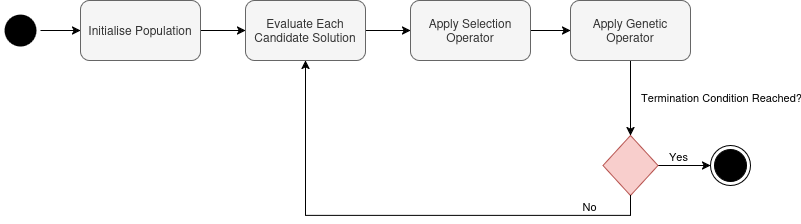
\includegraphics[width=\textwidth]{Figures/chapter_ea/chapter_ea_ea_framework.png} % Include the figure image
	\caption{Evolutionary Algorithm Framework (adapted from \cite{handsOnGeneticAlgorithms})}
	\label{fig:ea_framework} % Unique label used for referencing the figure in-text
\end{figure}

\subsection{Representation}
The term chromosome is often used to refer to representations of candidate solutions within the population which are a critical aspect of the evolutionary algorithms, an attempt to model genes and chromosomes seen in nature. The representation dictates how individuals are encoded, manipulated, and evaluated within the evolutionary process. A representation that is well-defined within the context of the optimisation problem enhances the algorithm's ability to explore the search space efficiently while maintaining diversity and feasibility among solutions.

\parbreak

\noindent The genotype-phenotype mapping translates encoded information into a meaningful solution. There are two forms in an evolutionary algorithm, namely, the \textbf{genotype} which is the encoded representation of a solution and is typically manipulated directly by genetic operators such as crossover and mutation, and the \textbf{phenotype} which is the decoded, functional representation of the solution which is what gets evaluated against the fitness function or objective (\cite{okramergeneticalgorithms}). For example, consider an optimisation problem where a 4-bit binary number that decodes the highest integer value needs to be found. The genotype would be a chromosome representing a 4-bit string (e.g., $1010$). The phenotype would be the decoded integer value (e.g., $1010 \rightarrow 10$ in decimal). It is not necessarily for every optimisation problem to have an explicit genotype-phenotype mapping, in particular, when the genotype is the solution itself (\cite{okramergeneticalgorithms}).

\parbreak

\noindent There are many ways in which chromosomes can be represented as solutions to the problem at hand. Representations are divided into two categories, namely, direct representations and indirect representations. Direct representations are those in which the genotype-phenotype mapping is one-to-one, allowing genetic operators to be applied directly without transformation. In contrast, indirect representations require an additional decoding step to map genotypes to phenotypes before genetic operators can be applied (\cite{rothlauf2009representations}). Genetic algorithms have originally been proposed to be binary coded to mimic the genetic material of natural organisms, however, different representations are used based contextually on the optimisation problem at hand (\cite{yu2010introduction}). Common representations include those seen in Figure \ref{fig:ea_representations}. Binary representations are commonly used for problems with discrete or combinatorial solutions, such as feature selection or Boolean optimisation, where each bit can encode the presence/absence of a feature or a binary decision. Integer or real-valued representations are suited for numerical optimisation tasks, such as parameter tuning in machine learning or engineering design, where variables require fine-grained precision. Tree-based representations model hierarchical structures, making them ideal for symbolic regression, program synthesis, or parsing tasks, where solutions naturally map to decision trees or recursive expressions.

\begin{figure}[h!] % Use [H] to suppress floating and place the figure/table exactly where it is specified in the text
	\centering % Horizontally center the figure on the page
	\includesvg[width=\textwidth]{Figures/chapter_ea/chapter_ea_representation.svg} % Include the figure image
	\caption{Common Gene Representation (adapted from \cite{intelligentOptimization})}
	\label{fig:ea_representations} % Unique label used for referencing the figure in-text
\end{figure}

\subsection{Population and Fitness}
The starting point in any evolutionary algorithm is the initialization of a population as shown in Figure \ref{fig:ea_framework} which represents a group of candidate solutions that could potentially solve the problem at hand. Unlike traditional optimisation techniques which mainly focus on a single-solution pathway, EAs work within the entire solution space by means of parallelism (\cite{okramergeneticalgorithms}). To put it simply, each generation evaluates candidate solutions as potential answers, with the algorithm progressively identifying better ones through selection and variation. This parallel search ensures that local optima are avoided, an issue which high-dimensional optimisation typically face. By ensuring that the initial population generated is diversified, there is an increased chance of finding a global or near global optimal solution. There are many methods for initializing a population, with randomized approaches being the most common, specifically those drawn from a uniform probability distribution, to ensure a broad coverage of the search space (\cite{initialPopulation}). Other mechanisms for initializing the population include heuristic and intelligent based approaches when existing solutions are known which could potentially ensure a better coverage spread of the search space (\cite{initialPopulation}). When taking advantage of using existing solutions to explore the search space, repetitive computations are mitigated yielding in an increased efficiency. Likewise, non-random initial populations can directly gear the algorithm to search a particular region of the solution space from the beginning which again, with the aid of known solutions, can allow the algorithm to converge quicker towards an optimal solution. Other mechanisms include deterministic based approaches in which candidate solutions are generated in a more controlled and evenly distributed manner leading to a better coverage of the solution space (\cite{THARWAT2021100952}).

\parbreak

\noindent In genetic algorithms, diversity refers to the variety of genetic material (e.g., different solution features or values) within a population. The population's diversity closely relates to how well the candidate solutions explore the search space. If individuals are too similar, they lack diversity leading to premature convergence causing stagnation around a suboptimal solution. Conversely, if the individuals are too diverse from one another, convergence can be delayed meaning that more generations are needed in order to hone in on an optimal solution (\cite{okramergeneticalgorithms}). A fine balance is therefore needed between exploration and exploitation. A highly diverse initial population is crucial to ensure thorough exploration of the search space early in the optimisation process. As generations progress, the algorithm selectively converges toward higher-quality solutions, naturally reducing diversity while refining the best candidates. There are well studied mechanisms which can control this balance such as mutation rate adjustment, niche-reserving mechanisms, or even hybrid approaches. Using these mechanisms ensures that both diversity and convergence can be capitalized.

\parbreak

\noindent With reference to Figure \ref{fig:ea_framework}, after the population is initialized, each candidate solution will be vetted by means of a fitness function which is a mathematical measure that scores how well the candidate solution meets the objective (\cite{okramergeneticalgorithms}). \todo[color=yellow]{"The fitness function needs to be discussed much earlier than this" $\rightarrow$ I am trying to follow the thought process of Figure \ref{fig:ea_framework} by following the flow diagram. I thought this may be easier to introduce for the reader.} This score reflects the quality of the candidate solution in regard to the optimisation goal and is used to guide the selection process in subsequent generations. For example, given an optimisation problem such that $x$ is an integer to maximize the parabolic equation $f(x) = -x^2 + 25$, the fitness function would be taking a candidate solution, and feeding it as input into this equation. Evidently, the maximum fitness to this function would be $5$. Fitness functions are defined in different ways depending on the application at hand, for example, in engineering design problems, fitness may represent efficiency, structural stability, or cost-effectiveness, whereas in artificial intelligence, fitness could measure a predictive accuracy. The way in which a fitness function is defined shapes how effectively the EA converges towards an optimal solution, especially in multi-objective problems (MOPs) where the fitness needs to account for multiple goals (\cite{book_introduction_to_evolutionary_computing}).

\parbreak

\noindent MOPs are mathematical problems that involve optimizing multiple conflicting objectives at the same time. The fitness function in this regard is defined by the algorithm's performance in relation to these conflicting objectives as opposed to one (\cite{okramergeneticalgorithms}). A common approach in formulating the fitness function is by aggregating all the objectives in a singular fashion by means of a weighted sum (\cite{okramergeneticalgorithms}). Another approach in defining the fitness function appropriately is by changing the structure of algorithm by means of co-evolution - instead of evolving a single population, the problem is broken down into smaller problems which in turn have their own population which is evolved (\cite{ZHOU201132}). In multi-objective optimisation problems which are common in economics and engineering, the fitness function may use methods like Pareto front optimisation which balances competing objectives without forcing single trade-off solutions. Pareto optimality describes a solution that cannot be improved in any objective without degrading another. In these kind of scenarios, EAs evolve a population of solutions that collectively represent a spectrum of optimal trade-offs, giving the decision-maker flexibility in choosing the most suitable solution based on contextual priorities (\cite{rachmawati2009multiobjective}). EAs are therefore robust and versatile in solving both single and multi-objective problems which can often be riddled with narrowly defined and complex optimisation challenges.

\subsection{Genetic Operators}\label{label:ea_genetic_operators}
In EAs, genetic operators - crossover and mutation - serves as crucial mechanisms by means of variation and adaption to guide the exploration of the solution space while refining existing solutions. Variation in evolution can be divided into two types based on their arity, namely, unary (mutation) and n-ary (recombination) both of which produce offspring (\cite{book_introduction_to_evolutionary_computing}). These operators mimic the evolutionary processes seen in nature among organisms, where gene recombination and mutation introduce new traits that contribute to a population's overall fitness and adaptability (\cite{handsOnGeneticAlgorithms}).

\subsubsection{Crossover}
Crossover is an evolutionary process based on sexual reproduction whereby genetic material from two parents are combined to produce offspring that inherit characteristics from both (\cite{okramergeneticalgorithms}). Crossover plays a crucial part in diversifying the algorithm's search path by combining beneficial traits and thereby ideally producing offspring with improved fitness. There are different ways in which crossover can occur which provide varying levels of control over the inheritance process. For simplicity, consider linear gene representations for the following crossover mechanisms:

\parbreak

\noindent \textbf{Single-point Crossover} selects a single point along the chromosome and exchanges genetic material on either side as shown in Figure \ref{fig:singlepoint}. This simple approach works well when minor structural adjustments results in significant improvement (\cite{intelligentOptimization}).
	
\begin{figure}[H] % Use [H] to suppress floating and place the figure/table exactly where it is specified in the text
	\centering % Horizontally center the figure on the page
	\includesvg[width=\textwidth]{Figures/chapter_ea/chapter_ea_singlepoint.svg} % Include the figure image
	\caption{Single-point crossover}
	\label{fig:singlepoint} % Unique label used for referencing the figure in-text
\end{figure}

\noindent \textbf{Multi-point crossover} introduces more than one cutoff point, allowing for more complex combinations of genetic material from each parent thereby creating a more diverse offspring as shown in Figure \ref{fig:multipoint} (\cite{crossoverMethods}). Multi-point crossover is typically used in scenarios that are non-linear. 
	
\begin{figure}[H] % Use [H] to suppress floating and place the figure/table exactly where it is specified in the text
	\centering % Horizontally center the figure on the page
	\includesvg[width=\textwidth]{Figures/chapter_ea/chapter_ea_multipoint.svg} % Include the figure image
	\caption{Multi-point crossover}
	\label{fig:multipoint} % Unique label used for referencing the figure in-text
\end{figure}

\noindent \textbf{Uniform crossover} selects each gene randomly from one of the corresponding genes of the parent as shown in Figure \ref{fig:uniform} (\cite{crossoverMethods}). This technique produces highly diversified offspring and is suitable when seeking greater diversity in the population thereby leveraging exploration.
	
\begin{figure}[th] % Use [H] to suppress floating and place the figure/table exactly where it is specified in the text
	\centering % Horizontally center the figure on the page
	\includesvg[width=\textwidth]{Figures/chapter_ea/chapter_ea_uniform.svg} % Include the figure image
	\caption{Uniform crossover}
	\label{fig:uniform} % Unique label used for referencing the figure in-text
\end{figure}

\noindent In scenarios where problem requirements are specific, crossover strategies can be tailored to meet particular constraints. For example, order crossover (OX1) is useful for optimisation problems such as the traveling salesman problem whereby maintaining certain order relationships between genes (cities) is critical (\cite{tsp}). Such customized crossover methods ensure that the offspring retain problem-specific constraints while still inheriting the most desirable traits from parent solutions. Beyond sexual recombination, horizontal gene transfer (HGT), inspired by bacterial gene exchange, can also diversify populations by transferring genetic material directly between solutions without parent-offspring relationships (\cite{hgt}).

\subsubsection{Mutation}\label{sec:ea_mutation}
Mutation in contrast to crossover introduces randomness in the algorithm by altering one or more genes in an individual's chromosome in order to create new traits and variation (\cite{evolutionaryComputingAndNeuralNetworks}). Mutation serves as the primary source of diversity within the population and important when solutions begin to become too familiar, a condition known as \textit{genetic drift} (\cite{advancesInEvolutionaryAlgorithms}). When individuals become too similar, this results in stagnation around suboptimal solutions causing convergence towards a local maxima. Mutation can occur in many ways, such as:

\parbreak

\noindent \textbf{Bit-flip mutation (aka bitwise mutation)} is applied to chromosomes represented in binary whereby each gene has a probability that its bit is inversed (changing from 0 to 1 or vica-versa) as shown in Figure \ref{fig:bitflip} (\cite{intelligentOptimization}).
	
\begin{figure}[H] % Use [H] to suppress floating and place the figure/table exactly where it is specified in the text
	\centering % Horizontally center the figure on the page
	\includesvg[width=\textwidth]{Figures/chapter_ea/chapter_ea_bitflip.svg} % Include the figure image
	\caption{Bit-flip mutation}
	\label{fig:bitflip} % Unique label used for referencing the figure in-text
\end{figure}

\noindent \textbf{Gaussian mutation} is applied to real valued chromosomes whereby a random gene is selected and a Gaussian distribution applied by means of the function below where $x_{i}^{i}$ is the offspring, $\sigma$ is a fixed parameter for all variables, $[b_{i}, a_{i}]$ represents the range of random gene, $erf^{-1}$ represents the inverse of $erf$ which is the Gauss error function, defined by $erf(y) = \frac{2}{\sqrt{\pi}}\int^{y}_{0}e^{-t^2}dt$ (\cite{bell2022applicationsgaussianmutationself}, \cite{gaussianMutation}). Gaussian mutation allows for controlled but continuous alterations.
\begin{equation}
	x_{i}^{'} = \sqrt{2} \sigma(b_{i} - a_{i}) erf^{-1}(u^{'}i)
\end{equation}

\parbreak

\noindent \textbf{Inversion mutation} selects a subset of genes and inverts the position as shown in Figure \ref{fig:inversion}. This mutation scheme is useful in combinatorial optimisation problems where the specific arrangement of elements matters such as the travelling salesman problem (\cite{intelligentOptimization}).
	
\begin{figure}[H] % Use [H] to suppress floating and place the figure/table exactly where it is specified in the text
	\centering % Horizontally center the figure on the page
	\includesvg[width=\textwidth]{Figures/chapter_ea/chapter_ea_inversion.svg} % Include the figure image
	\caption{Inversion mutation}
	\label{fig:inversion} % Unique label used for referencing the figure in-text
\end{figure}

\noindent The parameters that govern genetic operators do not have to be static. There is more complex EAs, these parameters can be adjusted dynamically as the algorithm progresses. Adaptive mutation rates for example can be useful in maintaining diversity during later stages of the search when converging towards an optima is prioritized. Likewise, crossover rates could increase when diversity is low in order to ensure that favourable genetic material continues to recombine as the algorithm refines its search (\cite{meyer2007self}). In hybrid approaches, self-adaptive genetic operators are used whereby the parameters of mutation and crossover evolve and form part of the chromosome, allowing the EA to essentially learn optimal rates over time based on the fitness at hand (\cite{meyer2007self}). 

\parbreak

\noindent Hybrid approaches in genetic operators have become popularized due to its powerful nature. For example, memetic algorithms combine the typical genetic operators described above with local search techniques which allow candidate solutions to further refine the search space by means of exploiting problem-specific knowledge or heuristics (\cite{neri2012memetic}). This combination is useful in complex landscapes where small local improvements can lead to an increased fitness score after major variations have been introduced through crossover and mutation in individuals. Hybrid genetic operators can therefore enhance the EAs ability to explore local optima thoroughly while still retaining a broad search capacity.

\parbreak

\noindent There is a fine balance between crossover and mutation in the efficacy of EAs. Mutation ensures that the EA explores new possibilities and avoids premature convergence while crossover allows the search space's best regions to be explored by recombining favourable traits of candidate solutions. These operators form a dynamic balance between exploration and exploitation, equipping EAs with the necessary flexibility to solve complex and non-linear optimisation landscapes.

\subsection{Selection Mechanisms}\label{sec:selection_mechanisms}
Selection occurs in an evolutionary process in two instances - parent selection and survivor selection. Parent selection has its primary purpose in distinguishing individuals based on their quality in order to allow better individuals to become parents of the next generation (\cite{handsOnGeneticAlgorithms}). Survivor selection, similar to parent selection, aims to distinguish individuals apart based on quality. Parent selection occurs before variation operators are applied while survivor selection occurs after offspring are produced and evaluated against the fitness function (\cite{book_introduction_to_evolutionary_computing}). This selection mechanism mimics the natural selection seen in nature where animals with desirable traits have increased likelihood of producing better offspring - akin to this, candidate solutions with better fitness scores are more likely to produce better quality offspring to solve the objective at hand. An effective selection mechanism will ensure that there is a balance between promoting high-quality solutions whilst maintaining population diversity ideally driving the EA towards a global optimum. Below are common selection mechanisms that are typically used within evolutionary algorithms:

\parbreak

\noindent \textbf{Fitness-proportionate selection} which is one of the simplest yet most renowned selection methods. In this selection approach, each candidate solution's probability of being selected is proportional to its fitness score relative to the total fitness of the population (\cite{shukla2015comparative}). Mathematically, the probability that each individual is selected is given by the formula below where $f_x$ is the fitness of individual $x$ (\cite{shukla2015comparative}).
\begin{equation}
	p_x = \frac{f_x}{\sum^{n}_{i=1}f_i}
\end{equation}
This selection mechanism is computationally efficient ($O(n)$ complexity) and ensures that fitter individuals are more likely to survive and reproduce while still giving less fit individuals the chance to contribute and preserve genetic diversity thereby preventing stagnation. The most common implementation of this approach is \textit{roulette-wheel selection}, which assigns selection probabilities analogously to slots on a roulette wheel such that higher fitness solutions occupy larger wheel segments and thus have greater likelihood of being selected. Although this process is simple, this mechanism may suffer from genetic drift if highly fit individuals dominate which results in a loss of diversity in subsequent generations. This approach raises considerations about the \textit{takeover time}, that is, the number of generations required for the best candidate solution's genes to dominate the population under selection pressure alone. Short takeover times indicate strong selection pressure that may lead to premature convergence, while longer takeover times encourage diversity within the population at the cost of slower optimisation.

\parbreak

\noindent \textbf{Tournament selection} offers a more controlled selection mechanism which is done by firstly by selecting a subset of individuals based on random sampling. Each subset known as tournaments will have individuals compete and the strongest survive. The size of the subset or tournament impacts the selection pressure - larger tournaments increases the chances that the fittest individuals will dominate while smaller tournaments result in a more diversified selection pool of individuals (\cite{shukla2015comparative}). Tournament selection is computationally efficient ($O(n)$ complexity) and provides a simple way to adjust selection pressure making it a popular choice in EAs (\cite{shukla2015comparative}).

\parbreak
	
\noindent \textbf{Rank-based selection} addresses the limitations of the fitness-proportionate selection scheme by ranking individuals based on their fitness rather than their raw fitness score (\cite{mitchell1998introduction}). This would mean that individuals with exceptionally low fitness scores would have an increased chance to be selected, lowering the chances of genetic drift. This selection method has complexity $O(n log n)$ and maintains selection pressure without skewing the algorithm aggressively towards highly fit individuals which will allow a broad exploration of the search space (\cite{mitchell1998introduction}).

\parbreak

\noindent \textbf{Elitism} is a technique that is generally used with other selection mechanisms to ensure that the most fit solutions are preserved across generations. In this mechanism, a hall of fame is produced by taking the top $n$ individuals which are then carried to the next generation without modification guaranteeing that the best solutions are always kept (\cite{mitchell1998introduction}). This method essentially prevents the best solutions from being lost due to changes made by genetic operators thereby accelerating convergence. Although elitism speeds up the rate at which the algorithm will converge, it can lower diversity leading into premature convergence on a suboptimal solution (\cite{malik2014preventing}).

\parbreak
	
\noindent \textbf{Niche and speciation} techniques are employed to encourage diversity in specific traits by creating subpopulations, or niches within the larger population, however, may be computationally more taxing (complexity $O(n^2)$) as opposed to the aforementioned selection techniques (\cite{back2012handbook}). Speciation can be categorised into four types based on the geographical result that manifested the speciation (\cite{michaelCilliers}):
\begin{itemize}
	\item \textbf{Allopatric speciation} occurs when the population is divided and no interactions occur between the resulting sub\-populations. Over many generations, the groups start to diverge until they can be distinguished apart to form their own new species.
	\item \textbf{Peripatric speciation} occurs when a portion of the population migrates away, forming their own sub\-population. Unlike allopatric speciation, individuals from different sub\-populations can still interact with each other. Over successive generations, these groups diverge to become their own separate species.
	\item \textbf{Parapetric speciation} is the similar to peripatric speciation with the difference that some interaction can still occur between separated sub\-populations. Although the interaction between groups are limited, over time the groups can still diverge to create separate species.
	\item \textbf{Sympathetic speciation} occurs when a group forms within the population still occupying the same geographical space. Over many generations, the group is still likely to diverge to form part of a separate species, however, with the added benefit of interacting with the same pool of individuals during the selection and reproduction stages. 
\end{itemize}
	
\noindent Research has yielded many techniques in order to stimulate niching within evolutionary algorithms: \todo{Please cite some of the papers by Dr Michael Cilliers (one of my former students) and include a discussion of different types of speciation as well as epigenetic based approaches to managing diversity.}

\begin{itemize}
	\item \textbf{Fitness Sharing} which operates on the principle that fitness is a shared resource among individuals in an attempt to reduce redundancy within a population or search space (\cite{back2012handbook}).
	\item \textbf{Clearing} which is a mechanism whereby the top individuals per niche can take primary advantage of the resource of that particular niche (\cite{back2012handbook}).
	\item \textbf{The Islands Model} which is a mechanism inspired directly from organic evolution whereby the population is divided into multiple subpopulations and evolved independently. During evolution, gene information is exchanged between subpopulations in an attempt to encourage trait migration in order to exploit a subpopulations search space (\cite{back2012handbook}).
\end{itemize}

\todo{Please cite the work of Dr Michele Cullinan who has published on distributed island-based evolution}

\section{Types of Evolutionary Algorithms}\label{sec:ea_types_of_ea}
EAs cover a large set of a large set of optimisation approaches that share the fundamental principles of population-based search, genetic variation, and selection, mimicking evolutionary processes. These algorithms have morphed into distinct types each aimed to be used in a particular class of problems. Well known evolutionary algorithms include genetic algorithms, evolution strategies, genetic programming and differential evolution. While all follow the core principles of evolutionary processes, each type is uniquely structured to address specific challenges in optimisation, making EAs a versatile tool for solving for a many complex problems.\bigskip

\subsection{Genetic Algorithms}\label{sec:genetic_algorithms}
Genetic Algorithms (GAs) are one of the most well known types of EAs, initially formalized by John Holland in the 1970s (\cite{mitchell1998introduction}). In traditional GAs, candidate solutions are represented as chromosomes with binary gene values (bit strings), however, these have now been extended to include real values representations as well. These chromosomes undergo genetic operations like crossover and mutation to produce new offspring for subsequent generations. The basic genetic algorithm follows the following basic framework:

\begin{algorithm}[H]
	\caption{Basic Evolutionary Algorithm that Genetic Algorithms follow (\cite{back2012handbook})}\label{alg:basic_genetic_algorithm}
	\begin{algorithmic}[1]
	% \Ensure $y = x^n$
	\item Initialise population of individuals
	\item Evaluate all individuals  by fitness function
	\item \textbf{repeat}
	\item \quad Select individuals (parents) for reproduction
	\item \quad Vary selected individuals in randomized manner to obtain new individuals (offspring)
	\item \quad Evaluate offspring by fitness function
	\item \quad Select individuals for survival from offspring and possibly parents according to fitness
	\item \textbf{until} stopping criterion fulfilled
\end{algorithmic}
\end{algorithm}

\noindent Traditional optimisation algorithms typically struggle with high-dimensional or noisy problem spaces, however, EAs find their solution for a given problem by dynamically adapting their search pathways. Solving for the solution is similarly tautological making EAs favorable when confronted with complex, or poorly-defined problems where the normal traditional algorithms struggle to explore the solution space as intricately (\cite{intelligentOptimization}). \bigskip

\noindent GAs have been proven to be effective in both discrete and combinatorial optimisation problems where the solution space is vast and discontinuous (\cite{book_introduction_to_evolutionary_computing}). Due to the flexibility by which the chromosomes can be represented, GAs are widely used in engineering design, machine learning, and scheduling problems where they can efficiently explore and exploit the search space at hand which can be of varying complexity (\cite{back2012handbook}). \bigskip

\noindent One of the distinguishing features that GAs have to offer are their ability to handle discrete variables and constraints naturally. This is simply done by defining the individual chromosomes as a sequence of discrete numbers as shown in Figure \ref{fig:encoding}. This makes GAs highly suitable in applications such as resource allocation, routing, and other combinatorial problems that require search across many permutations (\cite{back2012handbook}). The use of crossover and mutation gives GAs the flexibility to explore the search space thoroughly while selection mechanisms help guide the algorithm towards good quality solutions. As mentioned, GAs are characterised as a kind of local search which are also hybridized with other techniques (such as memetic algorithms), to refine solutions and enhance the performance of the search. While genetic algorithms are used as a general purpose approach, they still run a risk of failure. When genetic algorithms are used in optimisation problems that lack detail and are represented poorly, the algorithms' performance is directly affected (\cite{back2012handbook}). \bigskip

\begin{figure}[H] % Use [H] to suppress floating and place the figure/table exactly where it is specified in the text
	\centering % Horizontally center the figure on the page
	\includesvg[width=\textwidth]{Figures/chapter_ea/chapter_ea_encoding.svg} % Include the figure image
	\caption{Different encoding schemes}
	\label{fig:encoding} % Unique label used for referencing the figure in-text
\end{figure}

\todo{I think you need to mention encoding real values into a binary chromosome by representing their sign,  mantissa, and exponent.}

\subsection{Evolution Strategies}
Evolution Strategies (ES) were developed by Hans-Paul Schwefel and Ingo Rechenberg in the 1960s, as a means for solving continuous optimisation problems in the engineering field (\cite{intelligentOptimization}). Unlike traditional GAs which typically use binary or discrete representations, ES uses real-valued vectors to represent solutions making them well-suited for optimizing real-valued parameters. Evolution strategies emphasize mutation as the primary genetic operator, applying random changes to solution vectors to generate offspring while crossover plays a less pivotal role (\cite{back2012handbook}). Evolutionary Strategies operates as follows: \bigskip

\begin{algorithm}
	\caption{Evolutionary Strategy Algorithm (\cite{back2012handbook})}\label{alg:basic_evolutionary_strategy}
	\begin{algorithmic}[1]
	% \Ensure $y = x^n$
	\item Initialise population of individuals
	\item Evaluate all individuals  by fitness function
	\item \textbf{repeat}
	\item \quad Select parents for reproduction uniformly at random
	\item \quad Vary selected individuals in randomized manner to obtain offspring
	\item \quad Evaluate offspring by fitness function
	\item \quad Select individuals from best ranks for survival
	\item \textbf{until} stopping criterion fulfilled
\end{algorithmic}
\end{algorithm}

\noindent ES differs from GAs in another fundamental way which is its self-adaptive approach to mutation. This self-adaption is achieved by evolving the strategy parameters alongside the chromosome, allowing ES to tune its search almost autonomously (\cite{back2012handbook}). ES has been proven effective in solving engineering design problems where precise adjustments to real-valued parameters are essential. Its ability to control balance between exploration and exploitation, especially in continuous and high dimensional search spaces makes ES a powerful tool for optimisation problems requiring fine-grain control (\cite{book_introduction_to_evolutionary_computing}). \bigskip

\subsection{Genetic Programming}\label{sec:genetic_programming}
Genetic Programming (GP) introduced by John Koza in the early 1990s, represents a unique branch of EAs that evolve tree-like structures as opposed to linear chromosomes of fixed string (\cite{koza1994genetic}). These trees represent executable programs, typically made up of mathematical functions, logical operations, or other computational expressions. GPs are suitable for optimisation problems such as symbolic regression, machine learning, or automated problem-solving. The main idea behind GPs are simple: evolve these program structures iteratively over generations through core evolutionary algorithm operations such as crossover, mutation, reproduction. A key distinction of GP is how fitness is evaluated which is by executing each candidate program on representative test cases with its performance directly determining its fitness value. \bigskip

\noindent GP's primary strengths are its flexibility and interoperability as it allows users to analyze and modify the resulting programs directly. GPs can be applied to generate models from regression problems, develop classification systems, or even design control systems in robotics (\cite{o2009riccardo}). For example, in symbolic regression, GPs evolve mathematical expressions that fit observed data, often discovering intricate relationships that traditional regression techniques struggle to formulate (\cite{koza1994genetic}). Additionally, GP has been applied in fields like finance, image analysis, and automated design, where evolving decision rules or functional expressions can produce valuable insights and practical solutions (\cite{o2009riccardo}). \bigskip

\noindent GP follows the same framework that was shown in Figure \ref{fig:ea_framework}. A population is firstly initialized which in GP sense is by means of producing randomized trees. In order to prevent trees that lack too much diversity and are far too complex, the \textit{ramped half-and-half} method is used whereby a fraction of the population is initialized with trees having a maximum depth of 1, another fraction having a depth of 2, and so on (\cite{back2012handbook}). Once a population is generated, the algorithm will go through the trivial evolutionary process of selection, mutation, crossover and reproduction. Genetic operators however vary vastly in the way they are applied compared to traditional GAs. For example, when crossover occurs, this is implemented by means of subtree replacement as shown in Figure \ref{fig:gp_crossover} where an entire subtree is exchanged with another to produce offspring. \bigskip

\begin{figure}[H] % Use [H] to suppress floating and place the figure/table exactly where it is specified in the text
	\centering % Horizontally center the figure on the page
	\includesvg[width=\textwidth]{Figures/chapter_ea/chapter_ea_gp_crossover.svg} % Include the figure image
	\caption{Genetic Programming Crossover (adapted from \cite{book_introduction_to_evolutionary_computing})}
	\label{fig:gp_crossover} % Unique label used for referencing the figure in-text
\end{figure}

\noindent Subtree mutation, on the other hand, replaces a randomly selected subtree with a newly generated one, introducing new expressions and broadening the search space as shown in Figure \ref{fig:gp_mutation}. \bigskip

\begin{figure}[H] % Use [H] to suppress floating and place the figure/table exactly where it is specified in the text
	\centering % Horizontally center the figure on the page
	\includesvg[width=\textwidth]{Figures/chapter_ea/chapter_ea_gp_mutate.svg} % Include the figure image
	\caption{Genetic Programming Mutation (adapted from \cite{book_introduction_to_evolutionary_computing})}
	\label{fig:gp_mutation} % Unique label used for referencing the figure in-text
\end{figure}

\noindent Crossover and mutation allow GP to navigate a wide variety of functional forms and solution pathways making it well suited for problems that benefit from structural flexibility such as symbolic regression or predictive models (\cite{back2012handbook}). \bigskip

\noindent One of the challenges that GP faces is in managing computational resources as evolving complex trees can be computationally intensive (\cite{koza1994genetic}). This means that large populations and lengthy expressions may require significant processing power making GPs slower than better suited evolutionary methods. There are many ways to counteract this, one of which is to limit the tree depth, however, come at the disadvantage of less diverse individuals (\cite{koza1994genetic}). More advance approaches include techniques such lexicographic parsimony pressure where selection is modified to prefer smaller trees only in situations where fitness remains the same (\cite{luke2002lexicographic}). Another challenge is the additional effort required in ensuring that the trees resulting from genetic operation are valid programs (\cite{koza1994genetic}).

\subsection{Differential Evolution}
Differential Evolution (DE) offers a distinctive approach to continuous optimisation problems, particularly suited for high-dimensional search spaces with real-valued parameters (\cite{storn1995differential}). Unlike GAs which rely heavily on crossover and mutation of binary-coded chromosomes, DEs strength lies in its vector-based mutation scheme. The way in which it works is as follows:

\begin{enumerate}
	\item For each parent in the population, a trial vector $u_i(t)$ is generated. This trial vector is generated using the following formula:
	
	\begin{equation}
		u_i(t) = x_{i_1} + \beta(x_{i_2}(t) - x_{i_3}(t))
	\end{equation}

	where $x_{i_2}(t)$ and $x_{i_3}(t)$ are randomly selected individuals such that $i \neq i_1 \neq i_2 \neq i_3$. $i_2$ and  $i_3$ are chosen based on uniform sampling, and $\beta \in (1, \infty)$ which is a scaling factor for controlling amplification (\cite{storn1995differential})

	\item After obtaining the mutated offspring which is the trial vector, crossover occurs which is implemented as follows:
	
	\begin{equation}
		x_{ij}^{'}(t) =
		\begin{cases}
			u_{ij}(t) \:\: if \:\: j\in J \\ 
			x_{ij}(t) \:\: otherwise
		\end{cases}
	\end{equation}

	where $x_{ij}^{'}$ is gene $j$ of chromosome $i$, and $J$ is the set of chosen perturbation points, which is essentially the set of trial vectors (\cite{storn1995differential}).
	
	\item Once the offspring is produced from the crossover operator, the evolutionary process continues over iterative generations until termination conditions are met. \bigskip
\end{enumerate}

\noindent DE's main advantage lies in its simplicity, requiring only a few parameters like the mutation scaling factor and crossover rate which makes it easy to implement (\cite{storn1995differential}). In addition, DE's efficiency with limited parameters make it feasible for use in high-stakes, real-time applications like control system design and power system optimisation, where quick convergence on reliable solutions is essential for maintaining system stability and performance (\cite{das2010differential}). \bigskip

\noindent Despite DEs strengths, there are challenges in balancing exploration and exploitation. For problems with highly complex landscapes, DE may converge slowly if its mutation factor is not carefully tuned (\cite{das2010differential}). Along with this, DEs reliance on population-based differences for mutation can lead to stagnation in situations where diversity is rather low. To address this issue, adaptive differential evolution (ADE) has been developed where mutation and crossover rates adjust dynamically to encourage exploration in later stages of the generation run (\cite{das2010differential}). Other variations of this algorithm, like multi-objective differential evolution (MODE) extends DE to handle multiple objectives simultaneously which produces a set of pareto-optimal solutions offering the user a range of trade-off options (\cite{xue2003pareto}). \bigskip

\noindent Both GP and DE illustrate its versatility within the field of evolutionary algorithms, each tailored to different use cases. While GP excels at evolving flexible and interpretable models for symbolic and algorithmic problems, DEs efficiency in continuous space make it ideal for high-dimensional, real-valued optimisation tasks. Likewise, in situations where computer programs need to be created to approximate an optimisation task, this is where GP shines. These algorithms showcase the adaptability of evolutionary principles to address a wide range of complex problems. \bigskip

\noindent EAs are particularly valuable for problems where evaluating solution quality is straightforward, but generating optimal solutions remains computationally difficult. For such problems, EAs provide an effective approach provided that:
\begin{enumerate}
	\item the candidate solution can be represented in a modifiable format (e.g., trees, graphs, or vectors)
	\item the search space permits incremental improvements through variation operators
\end{enumerate}

\noindent This contrasts with traditional methods that may require explicit gradients or problem-specific heuristics (\cite{intelligentOptimization}).


\section{Current Research}\label{sec:ea_current_research}
The field of evolutionary algorithms continues to evolve, driven by advances in computation power, new problem domains, and the growing demand for more robust optimisation tools. Key trends in the evolution of this field include adaptive algorithms, EAs integration with machine learning, and the application of EAs to large-scale systems. \bigskip

\noindent One promising direction is the development of self-adaptive algorithms that can dynamically adjust their evolutionary parameters during the optimisation process. These algorithms eliminate the need for manual tuning, which is often time\-consuming and problem-specific. Self\-adaptive mechanisms are particularly valuable in solving problems with dynamic environments, applications of which has seen to be used in scheduling problems and vehicle routing during traffic congestion (\cite{dulebenets2018self}, \cite{sabar2019self}). \bigskip

\noindent Another interesting area of research is EA's involvement in machine learning and artificial intelligence. Evolutionary algorithms are increasingly used to optimise hyperparameters, architectures, and training processes for machine learning models, such as deep neural networks (\cite{young2015optimizing}). Beyond neural network, EAs are finding applications in automating machine learning workflows, including feature selection, model selection, and algorithm design (\cite{nikitin2022automated}). \bigskip

\noindent With the rise of big data, evolutionary algorithms are being adapted to handle large scale datasets. Traditional EAs face computational challenges when applied to large-scale problems, but advancements in distributed computing, cloud-based frameworks, and GPU acceleration have enabled EAs deployment on massive datasets. EAs are being tailored to solve large-scale optimisation problem in fields such as energy distribution and supply chain, an example of which was its application to schedule the power of distributed systems (\cite{guzek2014multi}), and another to optimise an integrated system of bioenergy production supply chains (\cite{ayoub2009evolutionary}).

\todo{Try and find even more recent work.}
%------------------------------------------------

\part{Part Two}


\stopcontents[part] % Manually stop the 'part' table of contents here so the previous Part page table of contents doesn't list the following chapters

%----------------------------------------------------------------------------------------
%	BIBLIOGRAPHY
%----------------------------------------------------------------------------------------

\chapterimage{} % Chapter heading image
\chapterspaceabove{2.5cm} % Whitespace from the top of the page to the chapter title on chapter pages
\chapterspacebelow{2cm} % Amount of vertical whitespace from the top margin to the start of the text on chapter pages

%------------------------------------------------

\chapter*{Bibliography}
\markboth{\sffamily\normalsize\bfseries Bibliography}{\sffamily\normalsize\bfseries Bibliography} % Set the page headers to display a Bibliography chapter name
\addcontentsline{toc}{chapter}{\textcolor{ocre}{Bibliography}} % Add a Bibliography heading to the table of contents

\section*{Articles}
\addcontentsline{toc}{section}{Articles} % Add the Articles subheading to the table of contents

\printbibliography[heading=bibempty, type=article] % Output article bibliography entries

\section*{Books}
\addcontentsline{toc}{section}{Books} % Add the Books subheading to the table of contents

\printbibliography[heading=bibempty, type=book] % Output book bibliography entries

%----------------------------------------------------------------------------------------
%	INDEX
%----------------------------------------------------------------------------------------

% \cleardoublepage % Make sure the index starts on an odd (right side) page
% \phantomsection
% \addcontentsline{toc}{chapter}{\textcolor{ocre}{Index}} % Add an Index heading to the table of contents
% \printindex % Output the index

%----------------------------------------------------------------------------------------
%	APPENDICES
%----------------------------------------------------------------------------------------

% \chapterimage{orange2.jpg} % Chapter heading image
% \chapterspaceabove{6.75cm} % Whitespace from the top of the page to the chapter title on chapter pages
% \chapterspacebelow{7.25cm} % Amount of vertical whitespace from the top margin to the start of the text on chapter pages

% \begin{appendices}

% \renewcommand{\chaptername}{Appendix} % Change the chapter name to Appendix, i.e. "Appendix A: Title", instead of "Chapter A: Title" in the headers

%------------------------------------------------

% \chapter{Appendix Chapter Title}

% \section{Appendix Section Title}

% Lorem ipsum dolor sit amet, consectetur adipiscing elit. Aliquam auctor mi risus, quis tempor libero hendrerit at. Duis hendrerit placerat quam et semper. Nam ultricies metus vehicula arcu viverra, vel ullamcorper justo elementum. Pellentesque vel mi ac lectus cursus posuere et nec ex. Fusce quis mauris egestas lacus commodo venenatis. Ut at arcu lectus. Donec et urna nunc. Morbi eu nisl cursus sapien eleifend tincidunt quis quis est. Donec ut orci ex. Praesent ligula enim, ullamcorper non lorem a, ultrices volutpat dolor. Nullam at imperdiet urna. Pellentesque nec velit eget est euismod pretium.

%------------------------------------------------

% \chapter{Appendix Chapter Title}

% \section{Appendix Section Title}

% Lorem ipsum dolor sit amet, consectetur adipiscing elit. Aliquam auctor mi risus, quis tempor libero hendrerit at. Duis hendrerit placerat quam et semper. Nam ultricies metus vehicula arcu viverra, vel ullamcorper justo elementum. Pellentesque vel mi ac lectus cursus posuere et nec ex. Fusce quis mauris egestas lacus commodo venenatis. Ut at arcu lectus. Donec et urna nunc. Morbi eu nisl cursus sapien eleifend tincidunt quis quis est. Donec ut orci ex. Praesent ligula enim, ullamcorper non lorem a, ultrices volutpat dolor. Nullam at imperdiet urna. Pellentesque nec velit eget est euismod pretium.

%------------------------------------------------

% \end{appendices}

%----------------------------------------------------------------------------------------

\end{document}
